% threepennygui-Ht.tex
\begin{hcarentry}[updated]{threepenny-gui}
\label{threepenny-gui}
\report{Heinrich Apfelmus}%05/17
\status{active development}
\makeheader

Threepenny-gui is a framework for writing graphical user interfaces (GUI) that
uses the web browser as a display. Features include:

\begin{compactitem}
\item \emph{Easy installation.} Everyone has a modern web browser
  installed. Just install the library from Hackage and you are ready to go.
  The library is cross-platform.
\item \emph{HTML} + \emph{JavaScript}. You have all capabilities of HTML at
  your disposal when creating user interfaces. This is a blessing, but it can
  also be a curse, so the library includes a few layout combinators to quickly
  create user interfaces without the need to deal with the mess that is CSS. A
  foreign function interface (FFI) allows you to execute JavaScript code in
  the browser.
\item \emph{Functional Reactive Programming (FRP)} promises to eliminate the
  spaghetti code that you usually get when using the traditional imperative
  style for programming user interactions. Threepenny has an FRP library
  built-in, but its use is completely optional. Employ FRP when it is
  convenient and fall back to the traditional style when you hit an impasse.
\end{compactitem}

You can download the library from Hackage or Stackage and use it right away to
write that cheap GUI you need for your project. Here a screenshot from the
example code:

%**<img width=700 src="./chat.jpg">
%*ignore
\begin{center}
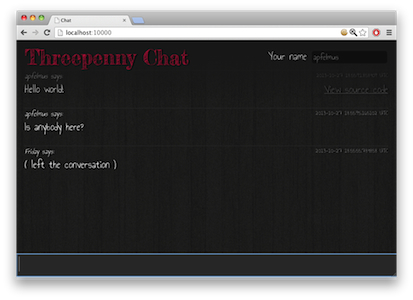
\includegraphics[width=\columnwidth]{html/chat.jpg}
\end{center}
%*endignore

For a collection of real world applications that use the library, have a look
at the gallery on the homepage.

\subsubsection*{Status}

The latest release is version \verb`0.8.2.0`. I would like to thank co-maintainer Simon Jakobi for his diligent and timely releases.

Compared to the previous report, several small additions to the API have been made, the documentation has been improved, and compatibility with the latest GHC versions has been ensured. Moreover, I given a tutorial about the library on HaL 2017, and the slides are now available in the source repository.

\subsubsection*{Future development}

The library is still in flux, API changes are likely in future versions.

In the future, I hope to improve the functional reactive programming (FRP) aspects of the framework, for instance by using the \verb`reactive-banana` library as a basis. \cref{reactive-banana}

\FurtherReading
\begin{compactitem}
\item Project homepage: \url{http://wiki.haskell.org/Threepenny-gui}
\item Example code:
  \url{https://github.com/HeinrichApfelmus/threepenny-gui/tree/master/samples#readme}
\item Application gallery: \url{http://wiki.haskell.org/Threepenny-gui#Gallery}
\end{compactitem}
\end{hcarentry}
